\documentclass[letterpaper,twocolumn]{article}
 
% Packages
\usepackage[utf8]{inputenc}
\usepackage{ragged2e} % Allows \RaggedRight for better control
\usepackage[margin=0.75in]{geometry}
\usepackage{graphicx}
\usepackage{hyperref}
\usepackage{url}
\usepackage{xurl}  % Enhanced URL breaking
\usepackage[numbers,sort&compress]{natbib}
\usepackage{needspace}

% Configure URL breaking
\def\UrlBreaks{\do\.\do\@\do\\\do\/\do\!\do\_\do\|\do\;\do\>\do\]%
  \do\)\do\,\do\?\do\'\do+\do\=\do\#\do\-}
\usepackage{float}
\usepackage{placeins}
\usepackage{multicol}
\usepackage{titlesec}
\usepackage[skip=3pt]{caption}
\usepackage{listings}
\usepackage[style=iso]{datetime2}
\usepackage{tabularx}

\captionsetup{font=small}  % Options: scriptsize, footnotesize, small

% Configure listings package 
\lstset{
  basicstyle=\ttfamily\small,
  frame=single,
  breaklines=true, 
  showstringspaces=false,
  columns=flexible
}

% Section title formatting
\titleformat{\section}{\normalfont\Large\bfseries\raggedright}{\thesection}{1em}{}
\titleformat{\subsection}{\normalfont\large\bfseries\raggedright}{\thesubsection}{1em}{}

% Page setup
\setlength{\columnsep}{0.25in}
\raggedbottom

% Enhanced widow and orphan prevention
\widowpenalty=15000        % Increased from 10000
\clubpenalty=15000         % Increased from 10000
\displaywidowpenalty=15000 % For math displays
\brokenpenalty=15000       % Discourages hyphenation across pages
\predisplaypenalty=10000   % Discourages breaks before displays
\postdisplaypenalty=10000  % Discourages breaks after displays

% Prevent single words on lines
\tolerance=1000
\emergencystretch=3em
\hbadness=10000
\vbadness=10000
\sloppy                    % Allows more stretch
\finalhyphendemerits=5000  % Discourages hyphenation in last line
\doublehyphendemerits=5000 % Discourages consecutive hyphens
\adjdemerits=5000          % Discourages breaks after short lines
\looseness=1              % Slightly looser spacing to prevent orphans

\hyphenpenalty=1000      % Increase penalty for normal hyphenation (higher discourages)


% Title and author information
\title{The Action Substrate:\\A Framework for Self-Sovereign Games and Communities}

\author{
Brent Fitzgerald \\
Matt Mason \\
Lex Johnson \\
Bryan Longhurst \\
Iaroslav Makarchuk \\
Oleksii Hodovanets \\
Oleksandr Vorobiov
 \\[1ex]
\texttt{team@basejump.xyz}
}

\date{DRAFT v0.7 - \DTMtoday}

% Configure list items to use RaggedRight
\newcommand{\configureRaggedItems}{%
  \let\olditem\item
  \renewcommand{\item}{\olditem\RaggedRight}%
}

\newcommand{\restoreItems}{%
  \let\item\olditem
}

\begin{document}


\maketitle
\configureRaggedItems

% Include sections

  

\begin{abstract}
The Action substrate is a decentralized framework designed to empower creators, incentivize participants, and establish sustainable digital economies. A network built on AO's decentralized compute layer, the Action substrate enables the creation and interoperability of sovereign worlds, games, game assets, and communities. At its core lies the ACTION token \ref{fig:action_token_symbol}, enabling interaction within the Action ecosystem, including governance participation, hyperobject creation, and economic coordination. Action prioritizes originality, collaboration, and sustainability, linking digital innovation to real-world impact through treasury-supported initiatives.
\end{abstract}
\vspace{1em}
\begin{figure}[ht]
  \centering
  
\includegraphics[width=0.35\columnwidth]{images/image1.png}
  \vspace{1em}
  \caption{The ACTION token}
  \label{fig:action_token_symbol}
  \end{figure}
\section{Background: Arweave and AO}

The Action substrate is built on AO, a revolutionary decentralized computing system that leverages Arweave's permanent data storage capabilities. To understand Action's architecture, it's essential to first grasp the foundational technologies it builds upon.

\subsection{AO: A Decentralized Computer}

Unlike traditional blockchains that operate as single-threaded systems with shared memory, AO functions as a decentralized computer that enables parallel execution of processes. This fundamental difference allows AO to support an unlimited number of concurrent processes without the scalability constraints typical of blockchain networks.

At its core, AO implements an actor-oriented paradigm where each process operates independently but can communicate through message passing\footnote{The actor-oriented paradigm in AO differs from traditional blockchain architectures by treating each process as an independent actor with its own state and behavior, rather than sharing a global state. This enables true parallel execution and eliminates the scalability bottlenecks common in traditional blockchain systems.}. This architecture creates a unified computing environment---a Single System Image---hosted across a distributed network of nodes. The result is a vast, scalable computer where users can interact with any process, fostering a highly collaborative ecosystem.

\subsection{Integration with Arweave}

AO uses Arweave as its persistent data layer, ensuring permanent availability of all process interactions and data. \cite{Williams2023} Rather than achieving consensus on computation results, AO ensures that logs of interactions are recorded and accessible on Arweave. This creates a `holographic' state system where the state may not have been computed by any participant yet but is guaranteed to always produce the same outputs when computed. \cite{Williams2024}

\subsection{Core Components}

AO's architecture consists of several key components that work together to enable decentralized computation, as shown in Figure \ref{fig:ao_architecture}:

\begin{figure}[ht]
\centering
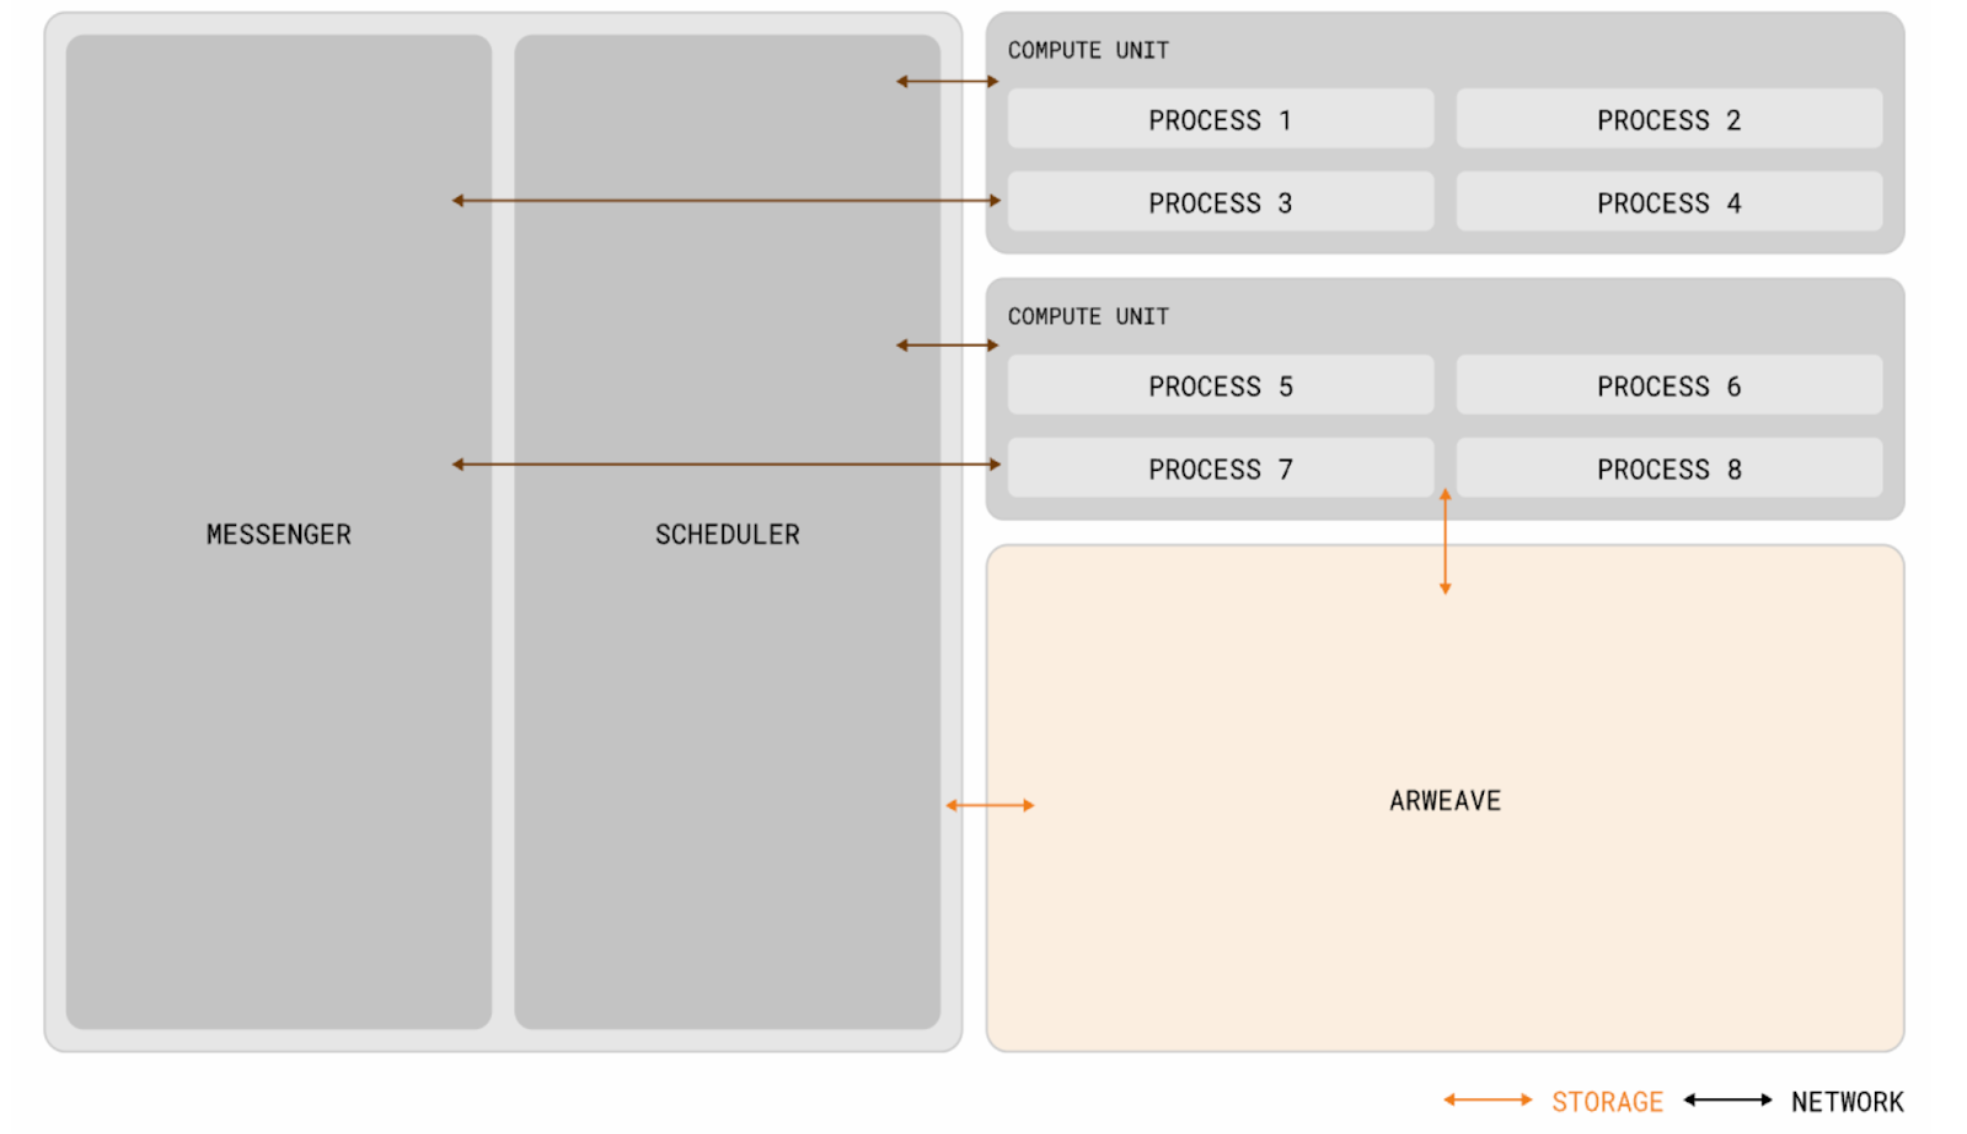
\includegraphics[width=\columnwidth]{images/image2.png}
\caption{The AO computer architecture takes a modular approach, splitting responsibilities into subnets where participants engage in peer-to-peer markets for service provision. \cite{Williams2024}}
\label{fig:ao_architecture}
\end{figure}

The fundamental building block is the \textbf{Process}, which represents the basic unit of computation in AO. Each process maintains a log of interacting messages stored on Arweave along with an initialization data item. Processes are highly configurable, defining their own computing environment including VM specifications, memory requirements, and necessary extensions.

\textbf{Messages} form the basis of all interactions within AO. Following the ANS-104 standard \cite{ANS104_2024}, messages are guaranteed to occur exactly once, with delivery confirmation ensured through Arweave's data persistence protocol\footnote{The ANS-104 standard ensures reliable message delivery through a combination of unique message IDs, cryptographic signatures, and Arweave's permanent storage. This guarantees that messages cannot be lost, duplicated, or tampered with, making it ideal for decentralized applications requiring strong consistency.}.

The system employs several specialized units to manage computation and communication. \textbf{Scheduler Units (SUs)} handle the critical task of assigning sequential slot numbers to messages sent to processes, ensuring proper message ordering and maintaining data persistence on Arweave. This orchestration preserves the integrity of all process interactions.

\textbf{Compute Units (CUs)} are responsible for calculating process states and providing signed attestations of computation results. These units operate within a peer-to-peer market, competing to offer computation services while balancing factors like price and performance.

\textbf{Messenger Units (MUs)} facilitate the relay of messages throughout the network, coordinating with both SUs and CUs to ensure proper message delivery and processing. These units also support advanced features like timed interactions and message subscriptions.

\subsection{Security Architecture}

AO employs a hierarchical and modular security model, allowing processes to tailor their security guarantees based on their specific needs. Security in AO is built on two fundamental pillars:

\subsubsection{Hierarchical Security}
Each process in AO operates independently, using a deterministically verifiable state model. Processes interact through cryptographically signed messages, relayed by Messaging Units (MUs). Each process has autonomy in defining its security model, enabling a range of trade-offs between latency, cost, and efficiency. This architecture ensures that security scales without requiring global verification, making AO highly adaptable.

\subsubsection{Economic Security}
AO's security is reinforced by economic incentives, primarily through the AO-Sec Origin staking mechanism. Participants can:
\begin{itemize}
\item Stake tokens to collateralize processes, with slashing mechanisms in place for malicious behavior
\item Sub-stake into custom security models, allowing more tailored security configurations
\item Leverage a market-driven approach where security is provisioned dynamically based on demand, akin to an open security insurance market
\end{itemize}

\subsubsection{Fallback and Byzantine Fault Tolerance}
AO ensures liveness and fault recovery by integrating with Arweave's Byzantine Fault Tolerant (BFT) consensus. This means that in case of node failures or process misbehavior, security can fall back to trustless verification mechanisms hosted on a decentralized and immutable ledger.

\subsection{AO Processes}

AO processes exhibit several unique characteristics that make them ideal for Action's needs:

\begin{enumerate}
\item \textbf{Unbounded Resource Utilization}: Processes can use unlimited computational resources, enabling complex applications like machine learning tasks and high-compute autonomous agents.
\item \textbf{Autonomous Activation}: Processes can have scheduled ``cron'' interactions that automatically trigger computation at set intervals.
\item \textbf{Modular Design}: Processes can specify their virtual machine, security parameters, and other operational requirements, allowing for maximum flexibility in application design.
\end{enumerate}

This architecture provides Action with a robust foundation for creating, managing, and securing digital assets and experiences. By building on AO, Action inherits the benefits of true decentralization, unlimited scalability, and permanent data availability, while adding its own layer of functionality specific to gaming and digital asset management.

\section{System Overview}

The core of the Action substrate is an object and experience layer running on the \textbf{AO compute network} \cite{Williams2024} and \textbf{Arweave} \cite{Williams2023} for persistence. Refer to Figure \ref{fig:system_overview} for a visual representation of the system.

\begin{figure}
  \centering
  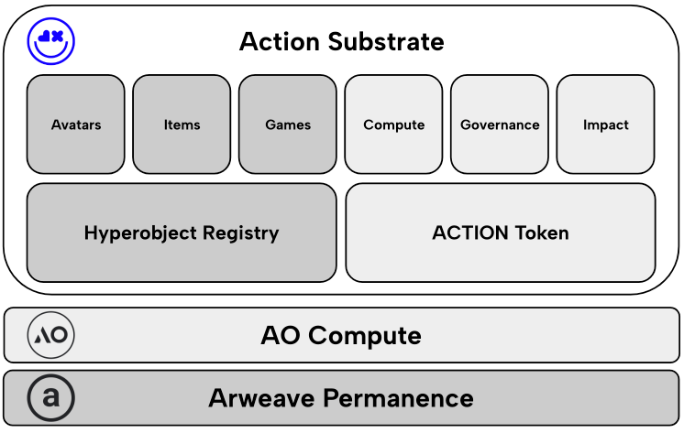
\includegraphics[width=0.95\columnwidth]{images/image3.png}
  \vspace{1em}
  \caption{ACTION runs on the AO Computer and Arweave, the global, permissionless hard drive.}
  \label{fig:system_overview}
\end{figure}

\textbf{Hyperobjects} are the foundational digital assets of the Action Substrate, serving as the building blocks for gameplay, commerce, and creativity across the ecosystem.

The \textbf{ACTION Token} allows for paying for Hyperobject creation and governance voting. Holder incentives are aligned around the expansion of robust, decentralized ecosystems built on game assets and engines. The main reason to acquire ACTION is to participate in the creation, gaming, or governance aspects, \textit{not} for speculative profit.

As the cost of creation continues to drop, Action reframes the value proposition around originality, collaboration, and community. By combining decentralized infrastructure with shared governance, it sets the stage for sustainable, vibrant communities, games and worlds built on the principles of creativity and ownership.

By integrating decentralized compute, AI-driven creation tools, and treasury-backed incentives controlled by the community, Action bridges the gap between digital innovation and real-world impact, supporting environmental and social initiatives through its governance mechanisms.


\section{Hyperobjects: The Building Blocks of the New Internet}

Simply put, hyperobjects are game assets such as avatars, items, and game environments that can be used across different games, chains, worlds, platforms, marketplaces, and connected IRL experiences, that form the foundation of in-game economies and interactions.

Hyperobjects share similarities with NFTs, but because of the scalability afforded by AO, an individual hyperobject can be a large application, such as a AAA game or AI agent, as opposed to a simple image. Players and creators can use hyperobjects to craft unique experiences, build new worlds, and participate in shared economies. Commonly used file types used for gaming, such as VRMs \cite{VRM2024}, GLBs, OBJs and USDZs\footnote{These file formats serve different purposes in 3D gaming and virtual worlds: VRM is optimized for humanoid avatars with standardized rigging, GLB/OBJ are general-purpose 3D model formats supporting meshes and textures, and USDZ is Apple's AR-optimized format. This diversity of formats enables hyperobjects to be compatible with a wide range of platforms and use cases.}, can be used as hyperobjects. Designed for interoperability, flexibility, and permanence, hyperobjects can be thought of as the hypertext of the gaming world in that they function as connective tissue---flexible, transferable, and useful across multiple platforms -- much like hypertext in the Internet we use today.

\subsection{Categories of Hyperobjects}

\subsubsection{Avatars (``Action Figures'')}
Action Figures serve as players' digital identities, representing their presence, abilities, and progression across different virtual worlds. These avatars are designed for full interoperability, functioning seamlessly across multiple games, social platforms, and streaming services while maintaining their skills, achievements, and personalized characteristics. 

Players can continuously evolve their Action Figures through customization and upgrades using other Hyperobjects, creating a persistent digital identity that spans the entire ecosystem.

\subsubsection{Game Assets (``Action Items'')}
Action Items are digital objects designed for use within games and virtual worlds. These items come in two main varieties, as illustrated in Figures \ref{fig:consumable_items} and \ref{fig:durable_items}: consumable items are one-time-use objects like power-ups, health packs, or crafting materials that are depleted upon use, while durable items are persistent assets such as weapons, tools, or collectibles that remain in the player's inventory and can be traded, upgraded, or staked over time.


\begin{figure}[t]
\centering
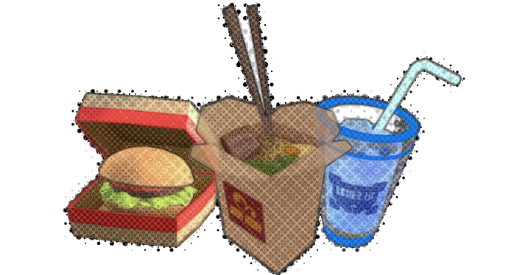
\includegraphics[width=0.9\columnwidth]{images/image4.png}
\vspace{1em}
\caption{Consumable Hyperobject: Action Items from the Basejump gaming platform boost an Action Figure's health when consumed, and can be used as melee weapons or projectiles in battle.}
\label{fig:consumable_items}
\end{figure} 



\begin{figure}[t]
\centering
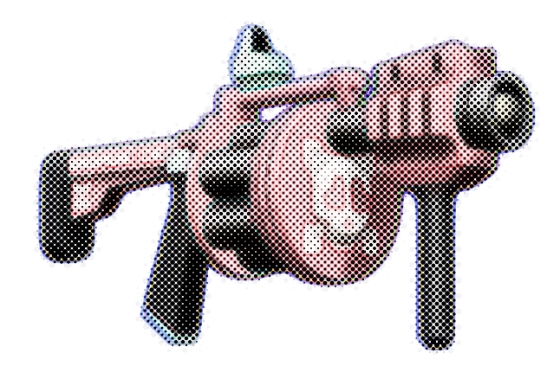
\includegraphics[width=0.8\columnwidth]{images/image5.png}
\vspace{1em}
\caption{Durable Hyperobject: An Action Item from the Basejump gaming platform (the EMP Glo-Stick Rocket Launcher) that exhibits context-dependent behavior: If used in web3 game Nifty Island, it fires bullets. In the battle game on Basejump, it fires glo-sticks.}
\label{fig:durable_items}
\end{figure}


\subsubsection{Game Environments (``Worlds'')}
\begin{itemize}
\item Maps, levels, and immersive environments that define the setting and rules of gameplay
\item Creators can publish and register Worlds using the Action substrate, ensuring interoperability with other assets
\end{itemize}

\subsection{Context-Dependent Behavior}

Hyperobjects exhibit \textbf{context-dependent behavior}, dynamically adapting to the specific game or world in which they are used. This ensures:

\begin{itemize}
\item \textbf{Defaults-first design}\footnote{Defaults-first design means hyperobjects come with pre-configured, sensible behaviors that work immediately in any compatible environment. This approach significantly reduces integration complexity for developers and ensures a consistent baseline experience, while still allowing for customization when needed.}: Hyperobjects ``just work'' in all environments with robust defaults, reducing onboarding friction
\item Developers can override or extend functionality through the Hyperobject Registry, introducing unique mechanics while maintaining interoperability
\end{itemize}

For example, the the Mutatio Fly (Figure \ref{fig:mutatio_fly}) is a piece of digital art that was turned into a drone Hyperobject in Basejump, allowing players to use it as a flying companion in the game

\begin{figure}[t]
  \centering
  
\includegraphics[width=0.7\columnwidth]{images/image5b.png}
  \vspace{1em}
  \caption{Giving existing game assets new utility as  Hyperobjects: Mutatio Flies released in Spring 2024 by XCOPY and Neon Glitch were given new utility in Basejump Winter 2024, where they can now also be used as drones that Action Figures can equip and use in the Basejump platform.}
  \label{fig:mutatio_fly}
\end{figure}
  
\begin{figure}
\centering
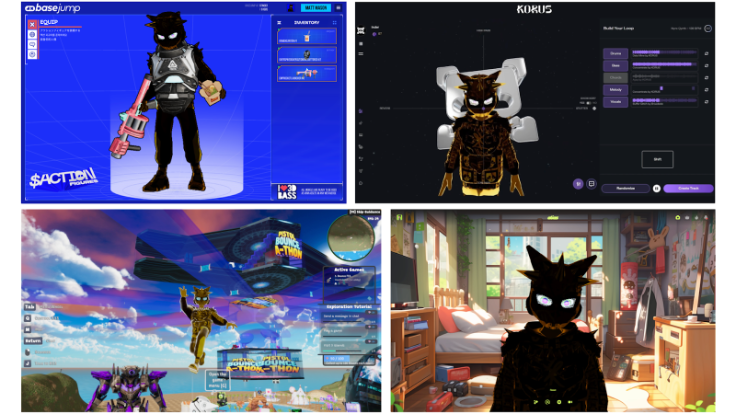
\includegraphics[width=\columnwidth]{images/image6.png}
\caption{An Action Figure hyperobject (Broadside OG 2969 - Stinger) exhibits context-dependent behavior in different platforms. Top Left: Stinger equipping EMP Glo-Stick Rocket Launcher and Ramen Action Items on Basejump. Top Right: Stinger working as a music-making companion in the AI music platform Korus. Bottom Left: Stinger functioning as a player avatar in Nifty Island. Bottom Right: Stinger performing as a live webcam avatar for 'v-tubing' in the Alias streaming video application.}
\label{fig:context_dependent}
\end{figure}

\subsection{Implementation}

The hyperobject design takes inspiration from some of the EVM ecosystem's primitives, such as the traditional ERC-721 (non-fungible) \cite{Entriken2018} and ERC-1155 (semi-fungible) \cite{Radomski2018} tokens, as well as newer standards like ERC-6551 (token-bound accounts) \cite{Windle2023}. The Action substrate also takes cues from other gaming protocols on EVM and elsewhere, such as Enjin \cite{Blagov2023}, Open Meta \cite{Gill2024}, Axie Infinity \cite{Nguyen2020}, and Immutable X \cite{Ferguson2021} among others. However, hyperobjects leverage AO's decentralized computer architecture, with each unique hyperobject running as a unique AO process with corresponding Arweave data representing its underlying assets. \cite{AtomicAsset}

The Hyperobject interface adheres to the AO community's developing process and token standards, including Atomic Assets \cite{AtomicAssetsSpec2024}, ANS-110 \cite{ANS110_2024} and ANS-103 \cite{ANS103_2024}. Figure \ref{fig:hyperobject_interface} shows the core interface methods that every Hyperobject implements.

\begin{figure}[t]
\begin{lstlisting}[basicstyle=\ttfamily\small]
-- Get info about the HyperObject process
Info() -> {
  Name, Creator, Metadata
}

-- Get balance of a specific account
Balance(Target?) -> {
  Balance, Ticker, Account, Data
}

-- Get all account balances
Balances() -> {
  Data -- JSON-encoded map
}

-- Get total supply of the Hyperobject
Total-Supply() -> {
  Action, Data, Ticker
}

-- Emits standard Credit-Notice and Debit-Notice
Transfer(Recipient, Quantity)

-- Callable only by the Hyperobject owner process
Mint(Quantity: string)

-- Callable only by a holder of the Hyperobject
Burn(Quantity: string)
\end{lstlisting}
\caption{Hyperobject Handler Interfaces (pseudocode): Core methods for querying state and performing transactions in the Hyperobject protocol.}
\label{fig:hyperobject_interface}
\end{figure}

\section{ACTION Token}

\subsection{Overview}

The main reason to acquire ACTION is to participate in the creation, gaming, or governance aspects, not for speculative profit.

\subsubsection{Purpose and Utility}
The ACTION Token represents \textbf{ownership} and \textbf{governance} within the Action Substrate. Core uses include:

\begin{itemize}
\item Paying for hyperobject creation, publishing, and registry
\item Facilitating transactions within the marketplace
\item Staking may be used for network security and participation in governance but does not provide financial returns\footnote{The staking mechanism is designed purely for network security and governance participation, not as an investment vehicle. Staked tokens are locked for governance voting power and network validation, but do not generate yield or financial returns, distinguishing ACTION from traditional yield-bearing tokens.}
\item Participating in governance to shape protocol updates and treasury allocations
\item Fostering community expansion and incentivizing activity on Action
\item Extensible utility. As game assets evolve, and the number of people using onchain game assets expands, and ACTION may be utilized in new ways by the community.
\end{itemize}

\subsubsection{Unique Value Proposition}
\begin{itemize}
\item Directly tied to the growth of sovereign worlds and games on the Action substrate
\item Incorporates treasury mechanisms to fund environmental and social initiatives
\item The Action substrate, leveraging AO's network, may further incentivize security and sovereignty by tying hyperobjects to validated node operation
\end{itemize}

\subsubsection{Implementation}
\begin{itemize}
\item Built and spawned on the audited AO token blueprint
\item Disowned by the deployer at launch
\item ACTION governance will transition over time through an autonomous governance framework, reducing reliance on any single entity
\end{itemize}

\subsection{Distribution and Allocation}

\textbf{Fixed Supply:} 10,000,000,000 ACTION\footnote{The fixed supply of 10 billion tokens was carefully chosen to balance sufficient granularity for microtransactions with the need to maintain scarcity. This number allows for broad distribution across the ecosystem while ensuring each token retains meaningful utility for governance and platform interactions.}

\vspace{0.5em}

\noindent The majority of ACTION tokens (75\%) will be allocated to the communities using Action, and the Broadside and Basejump communities that inspired its creation. Contributors and team receive allocations for contributing work to the ecosystem, not as passive investments expecting a return.


\begin{figure}
\centering
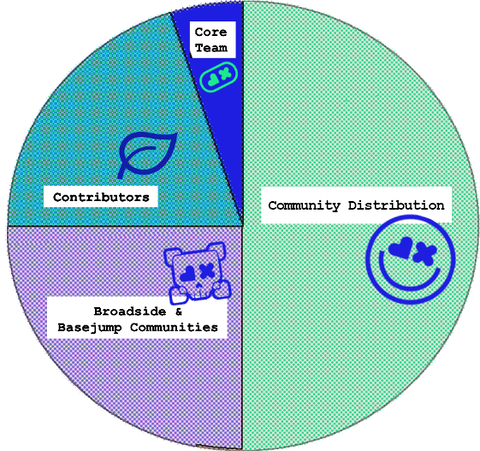
\includegraphics[width=0.8\columnwidth]{images/image7.png}
\vspace{1em}
\caption{ACTION Token Distribution and Allocation}
\label{fig:token_distribution}
\end{figure}

\begin{table}
  \centering
  \renewcommand{\arraystretch}{1.2}
  \caption{ACTION Token Distribution\protect\footnotemark}
  \begin{tabularx}{\columnwidth}{>{\raggedright\arraybackslash}p{0.7\columnwidth}>{\raggedleft\arraybackslash}p{0.2\columnwidth}}
  \hline
  \textbf{Category} & \multicolumn{1}{>{\raggedleft\arraybackslash}p{0.2\columnwidth}}{\textbf{Allocation}} \\
  \hline
  Community Distribution & 50\% \\
  Basejump \& Broadside Ecosystem & 25\% \\
  Contributor (future team, advisors, and investors) & 20\% \\
  Basejump Team & 5\% \\
  \hline
  \end{tabularx}
\end{table}
\footnotetext{Contributors and Team distributions are subject to one year lock and three year schedule}

\subsubsection{Community Distribution (50\%)}
\begin{itemize}
\item 50\% of ACTION tokens will be made available via the Permaweb Index; a new engine for community-driven distribution on AO designed to foster growth across the Permaweb
\item For more on the PermaWeb Index, visit \url{https://ao.arweave.net/}
\item The primary aim is broad usage and decentralization, \textit{not} raising capital
\end{itemize}

\subsubsection{Action, Basejump and Broadside Ecosystem (25\%)}
\begin{itemize}
\item 20\% of ACTION tokens will be reserved for Basejump users and communities, including the Broadside OG community, and allocated as rewards for playing games built on Action, creating new games and assets using Action, and for helping grow the Action ecosystem
\item 5\% of ACTION tokens will be allocated to Broadside OG holders
\item Broadside OGs will also earn the highest multipliers on rewards within the Basejump ecosystem
\item This allocation of ACTION will distribute directly to Broadside OG Action Figures
\end{itemize}

\subsubsection{Contributors (20\%)}
\begin{itemize}
\item We are setting aside 20\% of ACTION token supply for current and future contributors to the development of the Action ecosystem. This includes strategic partners such as Community Labs, as well as potential future contributors, team members and advisors. \cite{Takahashi2023}
\item Contributor allocations are subject to a one year lock and three year distribution schedule
\end{itemize}

\subsubsection{Basejump Team (5\%)}
\begin{itemize}
\item 5\% of tokens is reserved for the core Basejump team, as well as advisors
\item Team allocations are subject to a one year lock and three year distribution schedule
\end{itemize}




\subsection{Economic Model}

\subsubsection{Supply Dynamics}
Fixed supply; total supply is capped for functional reasons (like ensuring consistency across all participants)

\subsubsection{Protocol Fee Flows}
Marketplace fees, hyperobject publishing/registration, direct sales, and compute/persistence fees

\subsubsection{Feedback Loops}
Staking benefits, and usage-based demand tied to ecosystem growth

\begin{figure}[ht]
  \centering
  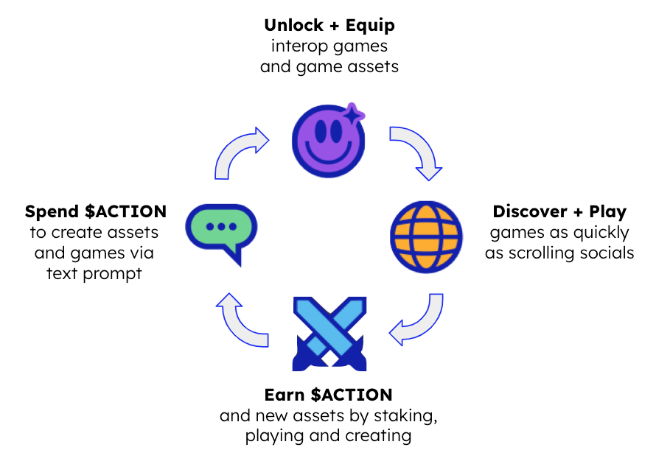
\includegraphics[width=\columnwidth]{images/image8.png}
  \caption{Action is an open-loop system, designed to reward users who play Action-powered games, create games and assets using Action, and help secure the network through staking.}
  \label{fig:economic_model}
\end{figure}
  

\subsection{Implementation}

ACTION's AO process is implemented according to the AO Token Blueprint, with the following standard handlers, as shown in Figure \ref{fig:action_token_interface}.

\begin{figure}[t]
\begin{lstlisting}[basicstyle=\ttfamily\small]
-- Get info about the ACTION token process
Info() -> {
  Name, Ticker, Logo, Denomination
}

-- Get balance of a specific account
Balance(Target?) -> {
  Balance, Ticker, Account, Data
}

-- Get all account balances
Balances() -> {
  Data -- JSON-encoded map
}

-- Emits standard Credit-Notice and Debit-Notice
Transfer(Recipient, Quantity)

-- Not implemented for ACTION
Mint(Quantity: string)

-- Get total supply of the token
Total-Supply() -> {
  Action, Data, Ticker
}

-- Callable only by a holder of ACTION tokens
Burn(Quantity: string)
\end{lstlisting}
\caption{ACTION Token Handler Interfaces (pseudocode): Core methods for querying state and performing transactions in the ACTION token protocol.}
\label{fig:action_token_interface}
\end{figure}

\section{Governance Framework}

A number of aspects of the Action substrate may be governed by token holders. In order to prioritize active individual community contributors over institutions, the governance protocol may employ mechanisms such as quadratic voting and sybil-resistant engagement metrics. 

As the network matures, the founding team's control over key decisions diminishes. The team aims for on-chain voting to exclusively govern treasury disbursements by Q1 2027.

\subsection{Voting Mechanisms}

The governance system employs multiple mechanisms to ensure fair and effective decision-making:

\vspace{1em}

\noindent\textbf{Quadratic Voting:} Following successful implementations like Gitcoin \cite{Gitcoin2023}, this mechanism balances influence by reducing outsized impact of large holders\footnote{Quadratic voting makes the cost of votes increase quadratically with the number of votes cast. For example, casting 1 vote costs 1 token, but casting 2 votes costs 4 tokens, 3 votes costs 9 tokens, etc. This ensures that a single large holder cannot dominate governance decisions, as the cost of additional votes becomes prohibitively expensive.}.

\vspace{1em}

\noindent\textbf{Engagement-Based Weighting:} Voting power is influenced by active participation in the ecosystem\footnote{The engagement-based weighting system uses on-chain metrics to measure meaningful participation, such as length of token staking, frequency of hyperobject creation/trading, and node operation uptime. This creates a meritocratic system where voting power is earned through sustained contribution to the ecosystem rather than just token holdings.}. Examples include:
\begin{itemize}
\item Stake tokens over time
\item Run an AO or Action node
\item Create or trade Hyperobjects
\end{itemize}

The community may further evaluate and migrate to other decisioning systems over time, allowing the protocol to evolve and adopt best practices in future.

The treasury also will utilize built-in constraints and guardrails to ensure allocations for environmental initiatives and ecosystem sustainability (Real World Action).

\section{Market Strategy}

\subsection{Adoption Plans}
\begin{itemize}
\item Launch the Basejump Battle Game (powered by Action) as a Discord and web game
\item Incentivize gamers to play games on Action by rewarding them both ACTION and hyperobjects, leveraging mechanisms such as invite-to-earn and play-to-earn
\item Incentivize creators and studios to publish hyperobjects and bring existing game assets to the Action substrate
\item Partnerships with decentralized platforms like AO and Arweave
\end{itemize}

\subsection{Exchange Listings}
Focus on DEX and CEX integrations with liquidity incentives. Strategic partnerships with exchanges will be prioritized to maintain alignment with Action's core values of sovereignty and decentralization

\subsection{Community Engagement}
Educational content, workshops, and collaborative initiatives to onboard participants, e.g. hands-on learning through game jams, creator workshops, and technical documentation to empower developers and creators to build on the Action substrate. 
\section{Background: Broadside and Basejump}

Action and the Basejump platform were inspired by the \href{https://opensea.io/collection/broadside/activity}{Broadside} community. Broadside began life in 2022 as an NFT project. The community that gathered around it quickly became one of the most active communities in the open metaverse. Watching how the Broadsiders came together to use blockchain connected assets across games, worlds and social platforms inspired the idea for hyperobjects and the Action substrate. As a result, the team behind Broadside created two key components to bootstrap development of the Action ecosystem:

\nopagebreak[4]
\begin{itemize}
\item The first collection of hyperobjects: Broadside OGs
\item The first application built on Action: Basejump
\end{itemize}


\begin{figure}
  \centering
  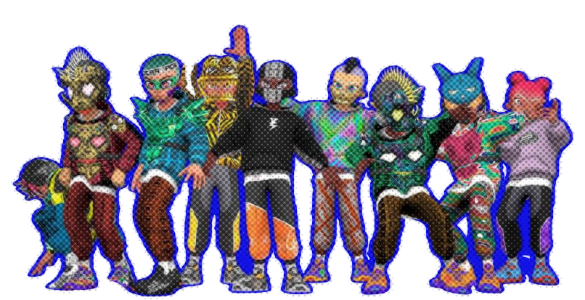
\includegraphics[width=\columnwidth]{images/image9.png}
  \caption{Broadside OG Action Figures, built using the VRM file format \cite{VRM2024}}
  \label{fig:broadside_og}
  \end{figure}

\subsection{Broadside OGs}

The Broadside OG collection has been converted to interoperable VRM \cite{VRM2024} avatars known as 'Action Figures' (Figure \ref{fig:broadside_og}) - concept cars designed to demonstrate the possibilities of hyperobjects that can:

\begin{itemize}
\item Unlock and use new Action Items, including weapons, clothing and armor
\item Earn the highest multipliers on both Basejump XP and ACTION
\item Feature AI text to speech functionality on Basejump in 300+ voices and 30 languages
\item Are compatible with thousands of experiences, worlds, games and platforms
\item Will continuously be upgraded with experimental new features
\end{itemize}


\subsection{Basejump}  

Basejump is a no-code surface that makes it easy to make, discover and monetize games and assets compatible with every platform, powered by the Action substrate.

\begin{itemize}
\item Most game creation platforms are toolsets. Basejump is a consumer focused, avatar-centric surface (Figure \ref{fig:basejump_platform}) with a deeply rewarding core game loop
\item Basejump's first core game (Figure \ref{fig:basejump_battle}) launches Spring 2025 on the web and natively in Discord
\item Basejump will be dropping new hyperobject collections with games, platforms, brands and artists designed to showcase hyperobject capabilities. Collaborations with Nifty Island and the Korus platform have driven early engagement, and a project with the hit Netflix show Black Mirror has been \href{https://x.com/blackmirror_xp/status/1786108170311541244}{announced}, in partnership with game studio Pixelynx
\item The Basejump creator hub is live now: \href{https://basejump.xyz/}{\texttt{basejump.xyz}}
\end{itemize}

\begin{figure}[t]
\centering
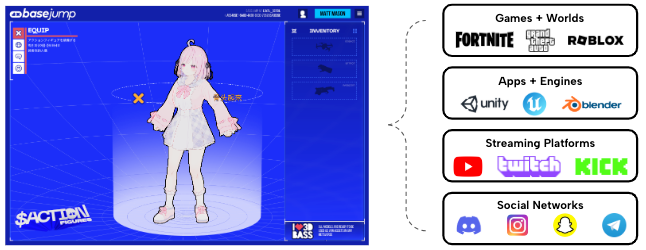
\includegraphics[width=\columnwidth]{images/image10.png}
\caption{Basejump makes it easy to make, discover and monetize games and assets compatible with every platform}
\label{fig:basejump_platform}
\end{figure}

\begin{figure}[t]
\centering
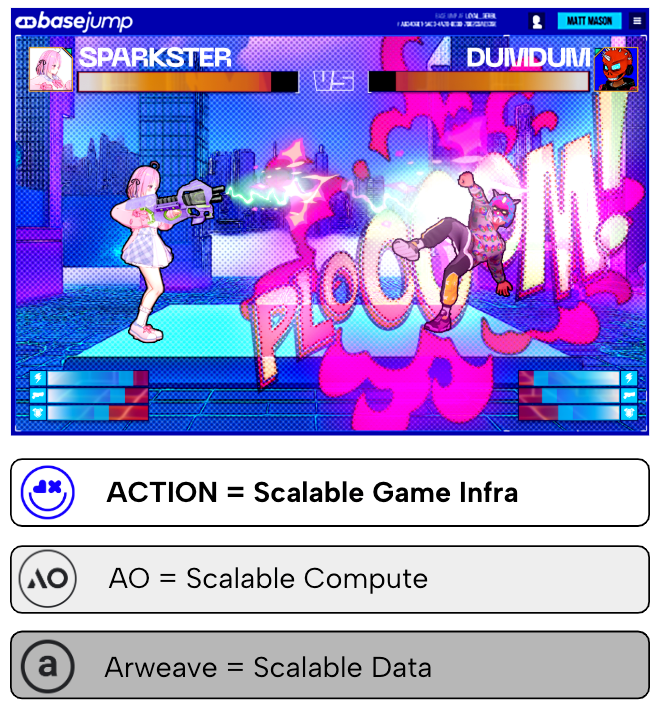
\includegraphics[width=\columnwidth]{images/image11.png}
\caption{Basejump runs as a PVP Battle game for hyperobjects in Discord and on the web, powered by Action, AO and Arweave.}
\label{fig:basejump_battle}
\end{figure}

\section{Action Figure Nodes}

The AO network provides decentralization and security by incentivizing diverse participants to participate as node operators

\begin{figure}[h]
  \centering
  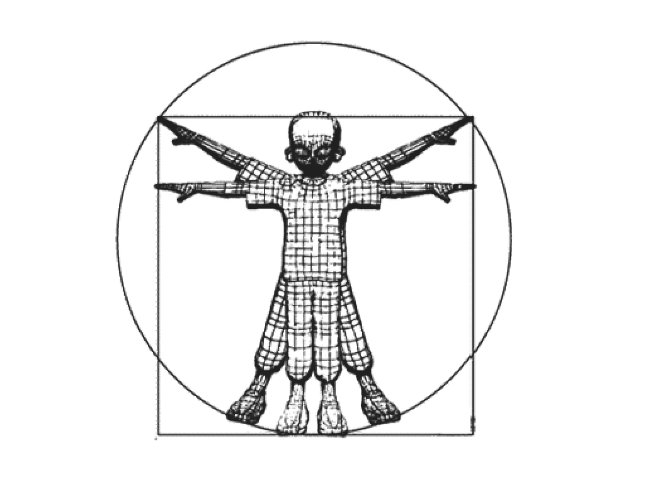
\includegraphics[width=\columnwidth]{images/image12.png}
  \caption{None of them are as strong as all of us: Connecting Action Figures to node operation at the UI level makes node operation more accessible, helps decentralize the Action substrate, and improves network security}
  \label{fig:action_figure_nodes}
\end{figure}

The Action substrate, leveraging AO's network, may further incentivize security and sovereignty by tying hyperobjects to validated node operation:

\begin{itemize}
\item Action's directional strategy is to eventually evolve to operate its own compute, with Action Figures (and potentially other hyperobjects) functioning as nodes
\item Nodes on AO can be customizable with devices and WebAssembly and can integrate with other services via relay device. Nodes on Action may be customized in certain ways, e.g. optimized for inference\footnote{Inference optimization would involve configuring nodes with optimizations (hardware and/or software) for AI/ML tasks. This includes using techniques like model quantization, parallel processing, and hardware acceleration to improve the performance of inference in processes.}
\item Broadside OGs will be the first Action Figures equipped with node functionality in our first experiments with this idea
\item By making Action Figures function as a 'front end' for nodes \ref{fig:action_figure_nodes}, node operation becomes more accessible to a larger cohort of users
\item Growing this community strengthens the security of the network
\end{itemize}

  
\begin{figure}
  \centering
  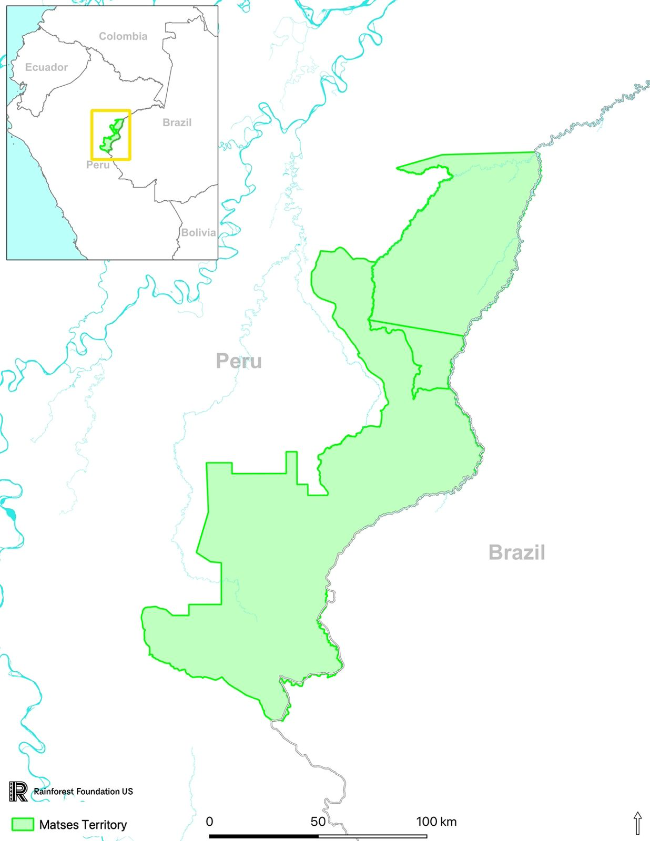
\includegraphics[width=0.9\columnwidth]{images/image13.png}
  \caption{The Matses territory --- an expansive area of nearly four million acres.}
  \label{fig:matses_territory}
\end{figure}

\begin{figure}
  \centering
  
\includegraphics[width=0.9\columnwidth]{images/image14.png}
  \caption{The Matses territory rendered as a live in-platform map in Basejump}
  \label{fig:matses_map}
\end{figure}

\section{Real World Action}

A percentage of fees earned from the minting of hyperobjects will protect a real-world area of rainforest. Working in partnership with Rainforest Foundation US\footnote{Rainforest Foundation US (RFUS) is a non-profit organization that works directly with indigenous communities to protect rainforests and secure their land rights. Since 1989, RFUS has helped indigenous communities protect over 33 million acres of rainforest across Central and South America through a combination of land titling, sustainable development, and technology-enabled monitoring.}, Basejump aims to protect nearly four million acres of Peruvian rainforest with the ACTION launch.

A portion of fees may be directed towards ecosystem grants, supporting real-world impact initiatives as voted on by the community, including support for Rainforest Foundation US' work safeguarding the Matses territory---an expansive area of around four million acres, as shown in Figure \ref{fig:matses_territory}.

Proceeds will be used to implement conservation and monitoring efforts, including the construction of small guard posts along key river tributaries\footnote{The guard post monitoring system combines traditional indigenous knowledge with modern technology. Local Matses community members staff strategically placed posts equipped with solar-powered communication systems, GPS units, and drones. This enables real-time monitoring of illegal activities while providing sustainable employment for indigenous communities \cite{RFUS2024}.}. These guard posts will help Matses communities monitor and regulate entry into their lands. Once the Matses territory is fully funded, we plan to expand our work with RFUS to additional regions.

As Action users create virtual worlds, we plan to scale efforts to protect the real world. By connecting gaming communities to real-world pieces of territory they can impact, Action is offering a new onchain, gamified framework for loose-knit communities to organize in new ways and solve complex problems, outside of (but working with) centralized organizations.

Non-profit organizations that allow donors to ``adopt'' a pet, project, or cause often yield better results in terms of donor engagement, retention, and emotional satisfaction. These programs often create a stronger emotional connection between the donor and the cause. Studies show that when donors feel a personal connection to a specific beneficiary (e.g., a named animal or project), they are more likely to give and continue supporting the cause. \cite{Small2003}

In the context of gaming, it's possible the Real World Action program can have a positive effect on player retention for games built on Action, leveraging blockchain to directly connect gaming communities to specific areas and real world communities that their efforts are helping protect, as visualized in Figure \ref{fig:matses_map}. Studies show that ``adopt'' programs often lead to higher donor retention rates because donors feel more involved and invested in the outcome. For example, receiving updates about ``their'' adopted animal or project can reinforce their commitment. \cite{Sargeant2004}

Specific, community-driven, gamified acts of protection can scale past our first experiment with Rainforest Foundation US. Over time the Action community can direct funding to a number of projects in this way, turning 'saving the world' into the world's greatest game.



\begin{figure*}[t]
  \centering
  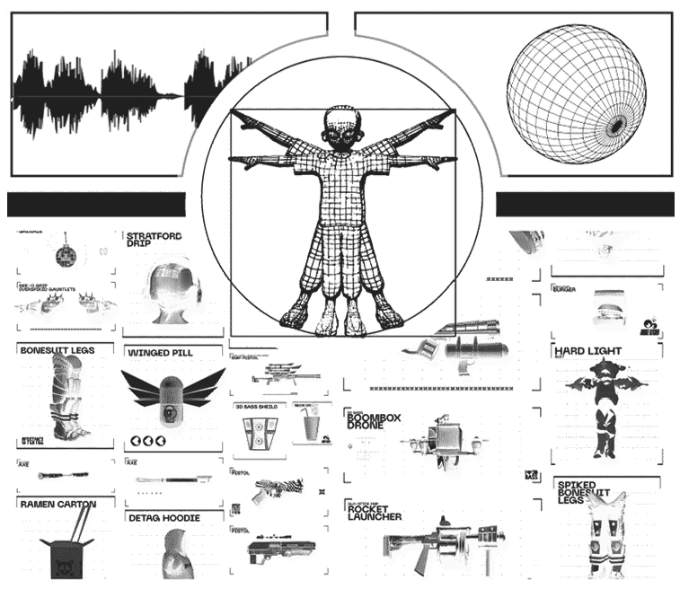
\includegraphics[width=0.9\textwidth]{images/image15.png}
  \caption{}
  \label{fig:vision}
\end{figure*}
\FloatBarrier % Prevents LaTeX from pushing content past this point
\section{Vision and Summary}

The Action substrate reimagines the digital economy for sovereign worlds, games, and communities. By combining decentralized infrastructure with creativity and shared governance, the protocol fosters originality, collaboration, and real-world impact.

\subsection{Key Highlights}
\begin{itemize}
\item \textbf{Hyperobjects}: Dynamic, interoperable assets - the connective tissue of the next Internet
\item \textbf{Action Substrate}: Decentralized compute and storage foundation
\item \textbf{ACTION Token}: Ownership, governance, and economic backbone
\item \textbf{Real World Action}: A solarpunk commitment to environmental and social good
\end{itemize}

Building on the scalable storage and compute made possible by Arweave and AO, Action aims to be a core layer of scalable gaming infrastructure for an Internet built on game engines, connected by game assets that are both interoperable and decentralized. Action sets the stage for a decentralized, collaborative metaverse built on the principles of creativity, ownership, and impact.

The Action ecosystem is designed to be a \textbf{utility-driven, decentralized framework} for self-sovereign gaming and digital asset interactions. By implementing \textbf{strong compliance measures, risk disclosures, and a structured governance transition}, Action aims to ensure \textbf{long-term sustainability and regulatory alignment}, mitigating potential legal and financial risks for participants.

\section{Regulatory Compliance Statement}

\emph{This document is for informational purposes only and does not constitute legal, financial, or investment advice. Prospective participants should conduct their own due diligence and consult with legal professionals before engaging with the Action ecosystem.}


\vspace{1em}  

ACTION is a utility token designed for use in the Action ecosystem and does not represent ownership, equity, or profit-sharing rights in any project or entity. Participation involves inherent risks, including technological, market, and regulatory uncertainties. Prospective participants are encouraged to conduct their own due diligence and consult professional advisors regarding any legal, financial, or tax obligations that may arise from holding or transacting with ACTION.

The Action ecosystem is committed to adhering to applicable U.S. laws and regulations, including securities, anti-money laundering (AML), and know-your-customer (KYC) requirements where necessary. While the ACTION token is designed as a \textbf{utility token} for use within the Action framework, we acknowledge that regulatory guidance on digital assets continues to evolve.

To ensure compliance:
\begin{itemize}
\item The \textbf{ACTION token does not represent equity} or ownership in any company, foundation, or affiliated entity
\item Token holders should not expect any return on their contributions
\item Regulatory frameworks are evolving, and tokens could be restricted or deemed subject to securities laws in certain jurisdictions
\item No guarantees can be made of liquidity or CEX / DEX exchange listings
\item The treasury mechanism is structured as a grant-based initiative, supporting ecosystem growth and community-selected projects without guaranteeing any form of return on investment to token holders
\item We will implement reasonable compliance measures, including potential KYC requirements for specific high-value transactions or governance participation where legally required
\item The project's governance transition will occur in a phased manner, progressively reducing reliance on the founding team and moving towards community-driven decision-making
\end{itemize}

\break
\section{Risk Factors and Disclaimers}

\subsection{Regulatory Risks}
The regulatory status of digital assets remains uncertain, and changes in laws or enforcement actions could impact the Action ecosystem
\begin{itemize}
\item The SEC and other regulators may assess the ACTION token's classification under the Howey Test or other securities laws
\item Tax implications may vary by jurisdiction, and users are encouraged to consult a qualified tax professional regarding their specific circumstances.
\end{itemize}

\subsection{Market Risks}
\begin{itemize}
\item The market value of the ACTION token may fluctuate significantly due to market conditions, demand, and adoption of the Action substrate
\item There is no guarantee that the ACTION token will maintain liquidity or be listed on any exchange, decentralized or otherwise
\end{itemize}

\subsection{Project Risks}
\begin{itemize}
\item Adoption of the Action substrate is subject to developer participation and user growth, and there is no guarantee of widespread adoption
\item Future enhancements, governance decisions, or network upgrades may introduce changes that affect token functionality or ecosystem incentives
\end{itemize}

\subsection{Decentralization and Governance Risks}
\begin{itemize}
\item While the Action ecosystem aims to transition toward decentralized governance, early-stage decisions will be made by the founding team to ensure operational stability
\item The governance structure will evolve over time, incorporating quadratic voting and engagement-based weighting to prioritize active community participation
\end{itemize}

\break
\section{Governance and Progressive Decentralization}
The Action ecosystem will implement a \textbf{phased approach to decentralization}, reducing reliance on the initial team while empowering community-driven governance over time.

\subsection{Phase 1: Early Governance \& Operational Control (Year 1-2)}
\begin{itemize}
\item Initial governance will be led by the Action founding team and key ecosystem contributors
\item Governance parameters, including treasury allocations and ecosystem incentives, will be established in consultation with the community
\end{itemize}

\subsection{Phase 2: Transition to Community Governance (Year 2-4)}
\begin{itemize}
\item Governance will transition to an \textbf{Action Foundation or DAO}, ensuring more distributed decision-making
\item The governance model may integrate \textbf{quadratic voting mechanisms} and weighted participation based on meaningful ecosystem contributions
\end{itemize}

\subsection{Phase 3: Fully Decentralized Governance (Year 4+)}
\begin{itemize}
\item The Action Foundation or DAO will have full control over protocol development, treasury allocations, and governance proposals
\item Core development teams will continue to support the ecosystem, but decision-making authority will be \textbf{fully vested in token holders and engaged participants}
\end{itemize}

\break
\section{Clarification on Treasury Mechanism}

The Action treasury \textbf{does not function as an investment vehicle} and does not distribute revenues or profits to token holders. The treasury's primary purposes are:

\begin{itemize}
\item \textbf{Ecosystem-building grants} to accelerate development of games, applications, and core infrastructure
\item \textbf{Developer incentives} to attract and retain talented builders in the Action ecosystem
\item \textbf{Real World Action} initiatives supporting environmental and social impact projects
\item \textbf{Operational sustainability} to ensure the long-term viability of the Action protocol
\end{itemize}

\noindent All treasury disbursements are:
\begin{itemize}
\item Subject to community governance decisions
\item Tracked through transparent reporting mechanisms
\item Aligned with ecosystem growth and community goals
\end{itemize}

\noindent\textbf{No portion of the treasury is distributed to token holders as a dividend, yield, or revenue share.}

\clearpage
\restoreItems
\raggedright
\bibliographystyle{unsrtnat}
\bibliography{references}

\end{document}
